\section{Plant/Condenser Loops}\label{plantcondenser-loops}

\subsection{Integration of System and Plant}\label{integration-of-system-and-plant}

In order to integrate the air handling system simulation with the zones simulation, methods were developed to model the system air loop and its interactions with the zones due to temperature controls and the relative difference between the zone and supply air temperatures. A similar situation is encountered when integrating the central plant simulation. Typically, the central plant interacts with the systems via a fluid loop between the plant components and heat exchangers, called either heating or cooling coils. In EnergyPlus the performance of the air systems and plant are interdependent because the simulations are combined. The plant outputs must match the system inputs and vice versa. That is, the temperature of the chilled water leaving the plant must equal the temperature of the water entering the coils, and the chilled water flow rate must satisfy mass continuity. In addition, coil controls are usually necessary to ensure that the values of chilled water flow variables entering and leaving the coil remain in a reasonable range. Plants can also interact with each other so that the operation of a chilled water loop and chiller will affect the operation of a condenser water loop.

\subsection{Current Primary System Modeling Methodology}\label{current-primary-system-modeling-methodology}

There are two main types of loops within the HVAC simulation in EnergyPlus: an air loop and a plant loop. The air loop is assumed to use air as the transport medium as part of an air handling system while the plant loops use a liquid fluid of the user's choosing (typically water).~ Condenser loops are a special case of plant loop that are for heat rejection and are distinguished by slightily different control options and applicable equipment types.~ A user may have any number of each type of loop in a particular input file. There are no explicit limits on the number of loops within the program---the user is only limited by computer hardware. Execution speed will naturally vary with the complexity of the input file.

Plant loops are further divided into ``half-loops'' or ``semi-loops'' for organizational clarity and simulation logistics (see Figure ``Connections between the Main HVAC Simulation Loops and Half-Loops''). These sub-loops, or half-loop sides, are matched pairs that consist of half of a main plant loop. Plant loops are broken into supply and demand sides. The plant demand side half-loop contains equipment that places a load on the primary equipment. This might include coils, baseboards, radiant systems, etc. The load is met by primary equipment such as chillers or boilers on the supply side half-loop. Each supply side half-loop must be connected to a demand side half-loop and vice versa. A similar breakdown is present on condenser loops where the demand side includes the water side of chiller's condensers while the supply side includes condenser equipment such as cooling towers.

\begin{figure}[hbtp] % fig 120
\centering
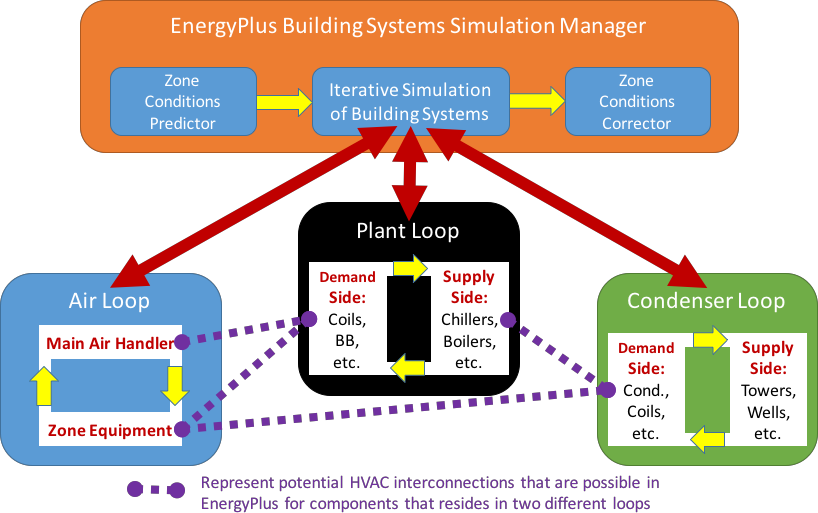
\includegraphics[width=0.9\textwidth, height=0.9\textheight, keepaspectratio=true]{media/image1957.svg.png}
\caption{Connections between the Main HVAC Simulation Loops and Half-Loops. \protect \label{fig:connections-between-the-main-hvac-simulation}}
\end{figure}

The breakdown into two half-loops allows for better handling and control of information and simulation flow throughout the program. Direct connections between the half-loops of the air, plant, and condenser loops are enhanced by components with connections between the various main loop types. For example, coils (heating or cooling) are in reality heat exchangers with an air and a water or refrigerant side. The air side of the coil is handled within the air loop where the control of the device is also maintained. The fluid side of the coil is handled within the plant demand side, which passes the energy requirements of the coil on to the plant supply side. All loops are simulated together by successively modeling each half-loop in a particulary calling order. Overall iterations ensure that the results for the current time step are balanced and updated information has been passed to both sides of the sub-loops as well as across to the other side of air loop connections such as coils.

The plant equipment on a half-loop is described by a set of branches for that half-loop.~ Components can be arranged on a branch in series, and branches can be placed in parallel, with some restrictions. Figure ``Branch Layout for Individual Plant Half-Loops'' provides an overview of the intended branch layout for each plant half-loop. Branches are individual legs within the loop structure. Thus, the segment between point A and point B is defined as a branch, as is the section between points E and F. There may be multiple sections (C1 to D1 through Cn to Dn) in between the splitter and mixer.

Each half-loop may only have one splitter and one mixer. Thus, equipment may be in parallel between the mixer and splitter, however, within any single branch, there can only be components in series and not in parallel. The topology rules for individual half-loops allow a reasonable amount of flexibility without requiring a complicated solver routine to determine the actual flow and temperature conditions. Note that since plant supply and demand are broken up into two separate half-loops, chillers or boilers may be in parallel to each other in the supply side and coils may be in parallel to each other on the demand side. Thus, the restriction of only a single splitter and mixer on a particular half-loop does not unduly limit the allowable configurations. In some cases a single branch can be used to define an entire half-loop, but in general a half-loop should have a splitter and a mixer even if all equipment on the sub-loop is simply in series.

In addition, to avoid the need for overly complex solver routines, there are some restrictions on the placement of pumps within a particular half-loop. There are two general types of pumps, loop pumps and branch pumps. A pump that is the first component on the first branch (between A and B) is termed a ``loop pump'' while any pump in the parallel section (between Ci and Di) is termed a ``branch pump''.~~ The simplest and most common arrangement is to have one loop pump on the supply side inlet.~ In plant demand half-loops pumps can be placed only in the inlet branch. This will allow simulation of primary-secondary systems. For more information on pumps and pump placement rules, see the section on PipingSystem:Underground Simulation Pumps in this document.

\begin{figure}[hbtp] % fig 121
\centering
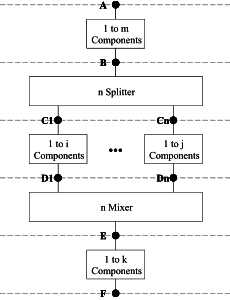
\includegraphics[width=0.9\textwidth, height=0.9\textheight, keepaspectratio=true]{media/image1958.svg.png}
\caption{Branch Layout for Individual Plant Half-Loops \protect \label{fig:branch-layout-for-individual-plant-half-loops}}
\end{figure}

Essentially, each branch is made up of one or more components linked together in series. The branch has system nodes that store properties at a location on the loop (temperature, enthalpy, flow rate, etc.) at the beginning and end of the branch as well as between components. Components on the branch take the conditions of the node at their inlet and use that information as well as overall control information to simulate the component and write the outlet data to the node following the component. This information is then used either by the next component on the branch or establishes the outlet conditions for the branch.

Although the plant model in EnergyPlus is quite flexible, in most cases the topology of the plant system in the model will be somewhat different from the topology of the actual plant system in a building.~ EnergyPlus is focused on modeling building energy performance over long periods of time and is not intended as a completely flexible system that can directly model any actual plant system with its full complexity and exact layout.~ Given the design of an actual complex plant system, the modeler will typically need to develop a simpler system that conforms to EnergyPlus's capabilities and strives to capture the issues important for energy consumption modeling.~ Just like complex geometry should be simplified into thermal zones for energy models, complex plants should to be simplified into sets of pairs of closed half-loops with the allowed branch topologies.

\subsection{Plant Manager}\label{plant-manager}

\subsubsection{Plant Half-Loop Calling Order}\label{plant-half-loop-calling-order}

Because there can be multiple plant loops in a model that depend on each other, one job of the plant manager is to determine an appropriate calling order for the half-loops.~ The intial starting calling order (and the order always used prior to EnergyPlus Version 7) is as follows:

1.~~~~Call all the demand side half-loops of the plant loops (in input object order)

2.~~~~Call all the supply side half-loops of plant loops (in input object order)

3.~~~~Call all the demand side half-loops of condenser loops (in input object order)

4.~~~~Call all the supply side half-loops of the condenser loops (in input object order).

This initial calling order is then revised during a setup phase of program execution when the plant component models are iteratively read in, initialized and sized.~ The algorithm is based on information provided by those component models that connect loops together.~ The components register that two loop-sides are connected and declare which one places demands on the other.~ If a half loop is connected and places demands on anther loop, then the calling order for the independent demanding loop is placed just ahead of the dependent loaded half-loop.~ For example a water cooled chiller component model reports that the supply side of the chilled water loop is connected to the demand side of the condenser loop and that the chilled water loop places demands on the condenser loop.~ The plant manger algorithm is iterative and repeatedly calls all of the half loops a total of four times.~ After this setup phase, the calling order is fixed for the rest of the simulation.

\subsection{Plant Flow Resolver}\label{plant-flow-resolver}

\subsubsection{Overview of the Plant Flow Resolver Concept}\label{overview-of-the-plant-flow-resolver-concept}

An important aspect of the solution procedure within plant loops is the method used to solve for the fluid flow rates throughout the various half-loops. This involves making the supply side meet a particular load and flow situation based on the simulation of the demand side loops. Load distribution is an issue that must be addressed as well as how flow rates are adjusted and temperatures are updated. These issues are discussed in the next several subsections, and the algorithms described are important to how the plant simulation functions.

In the first step, the plant loop manager calls the appropriate module to simulate (in flow order) all of the components on each branch of the loop except for splitters and mixers. In this step, each component would set the conditions at the outlet node including temperature, flow rate, maximum allowed (design) flow rate, minimum allowed (design) flow rate, maximum available flow rate, and minimum available flow rate. This would be based purely on the component's own control scheme and thus each component would be free to request as much (or as little) flow as desired.

In the second step, the loop manager would resolve the flow at all nodes and through all branches of the local loop. The components are then simulated with the corrected flows. For this iteration, the flow resolver sets the flow rate through each loop component.

\subsubsection{Overall Loop Flow Rate}\label{overall-loop-flow-rate}

The plant models determine an overall fluid flow rate for each loop based on the dynamic requests and needs of the components on the loop.~ The flow resolver examines the requests and needs of each half-loop and chooses an overall flow rate.~ As individual plant components are modeled, they register their requests for fluid flow which are stored on the inlet node (variable called MassFlowRateRequest).~~ These requests for flow are used for two purposes, overall loop flows and resolution of parallel flows inside a splitter/mixer.~ For determining the overall loop flow request, the requests by individual components are further qualified into three categories based on the nature of the device.

1.~~~~Need flow and turns loop on

2.~~~~Need flow if loop is already on

3.~~~~Take what ever flow they get.

The loop will only run at all if there are flow requests of type 1.~ If there are flow requests of type 2, they will not turn on the loop but may affect the overall flow rate if it is already on because of some non-zero type 1 requests.~ Flow requests of type 3 will not affect the overall loop flow rate.~ These classifications are hard coded and cannot be altered by the user.

\subsubsection{Pump Control for Plant and Condenser Loops.}\label{pump-control-for-plant-and-condenser-loops.}

The pump is quite simply the component that drives the flow (also see PipingSystem:Underground Simulation Pumps). . How it reacts depends on several different conditions. In total, there are three different decision variables, two of which are defined by user input. These three deciding factors are whether the pump is constant or variable speed, whether the pump operation is continuous or intermittent, and whether or not there is a request for overall loop flow. After the overall loop flow request has been determined the simulation knows what the loop would like to do.~ The next thing it does is simulation all the loop pumps to see what the pumps can actually provide. Then the overall loop flow is bounded by the minimum and maximum that the loop pumps can provide at that time. The operation of a constant speed pump is fairly straightforward. If the user designates a constant speed pump that is operating continuously, the pump will run regardless of whether or not there is a load. This may have the net effect of adding heat to the loop if no equipment is turned on. If the pump is constant speed and operates intermittently, the pump will run at its capacity if a load is sensed and will shut off if there is no load on the loop.

A variable speed pump is defined with maximum and minimum flow rates that are the physical limits of the device. If there is no load on the loop and the pump is operating intermittently, then the pump can shutdown. For any other condition such as the loop having a load and the pump is operating intermittently or the pump is continuously operating (regardless of the loading condition), the pump will operate and select a flow somewhere between the minimum and maximum limits. In these cases where the pump is running, it will try to meet the flow request for the overall loop.

In many cases, the first estimate of flow requested by the demand side tends to be fairly accurate and the flow rate does not vary in subsequent iterations. However, because there is the possibility that the coils or some other component might request more flow in future iterations during the same time step, the program must not only set flow rates but also maintain a record of the current maximum and minimum flow rate limits. This information is important not only to the pump itself but also to other pieces of equipment which may control their flow rates and thus require knowledge of the limits within which they may work. In general, the decisions on what to set the maximum and minimum flow rates is directly related to the type of pump (constant or variable speed). For constant speed pumps, the maximum and minimum flow rate values are the same and thus if the flow requested does not match this, the other components must either deal with the flow or a bypass branch must be available to handle the excess flow. For variable speed pumps, the maximum and minimum flow rates are set by the user-defined limits.

\subsubsection{Plant/Condenser Supply Side}\label{plantcondenser-supply-side}

Component models, such as boilers, chillers, condensers and cooling towers are simulated on the supply side of the plant and condenser loops. In order to allow specification of realistic configurations, the plant loop managers were designed to support parallel-serial connection of component models on the loop. In addition, loop managers were designed to support both semi-deterministic models (e.g.~the parameter estimation models of the ASHRAE Primary Toolkit {[}Pedersen 2001{]}) and ``demand based'' models (e.g.~the performance map models of BLAST and DOE2.1E). As a result, the loop manager must be able to simulate models that require the mass flow rate as an input and models that calculate the mass flow rate as an output---sometimes in the context of a single loop configuration.

In order to achieve these design criteria without resorting to a pressure based flow network solver in the HVAC portion of the code, a rules-based ``flow resolver'' was developed for the EnergyPlus plant manager. The flow resolver is based on the following assumptions and limitations:

\begin{itemize}
\item
  Each loop is only allowed to have a single splitter and a single mixer
\item
  Due to the fact that there can only be one splitter and one mixer on a given loop, it follows logically that there can be at most one bypass on each loop side
\item
  No other components may be in series with a bypass, i.e., a branch that contains a bypass may have no other equipment on that branch
\item
  Equipment may be in parallel only between the splitter and mixer components of a loop
\item
  Equipment may be hooked together in series in each branch of the loop
\item
  Flow rates on individual branches will be controlled using maximum and minimum available flow rate limits
\end{itemize}

The flow resolver employs a simple predictor-corrector algorithm to enforce mass continuity across the plant loop splitter as shown in the following figure.

\begin{figure}[hbtp] % fig 122
\centering
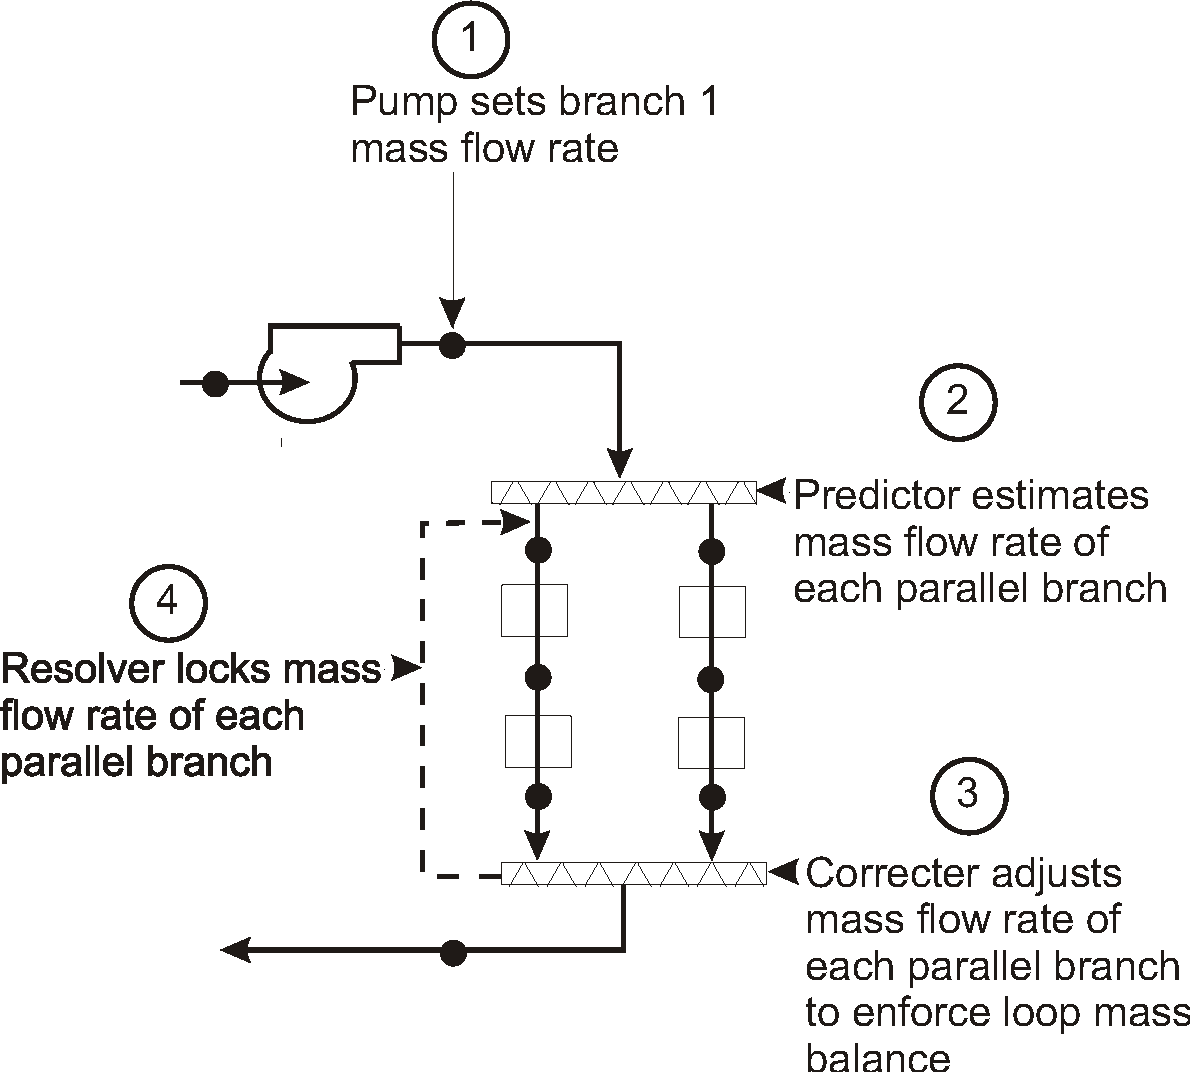
\includegraphics[width=0.9\textwidth, height=0.9\textheight, keepaspectratio=true]{media/image1959.png}
\caption{Plant/Condenser Supply Side Solution Scheme. \protect \label{fig:plantcondenser-supply-side-solution-scheme.}}
\end{figure}

As previously discussed, the pump establishes the total loop mass flow rate by setting the flow in the first supply side branch. In the second step, a predictor algorithm calls to simulate each piece of equipment on the loop and they update their mass flow rate requests based on the current flow rates, temperatures and load dispatch requests. The loop manager calls the appropriate module to simulate (in flow order) all of the components on each branch of the loop except for splitters and mixers. In this step, each component sets the conditions at its outlet node including temperature and sets component flows on the inlet node.~~ Each component and branch is classified for their type of flow control.~ Prior to version 7 this was input by the user where branch objects were tagged in the user input file as an ACTIVE, SERIESACTIVE, PASSIVE or BYPASS type of model.~ As of version 7 this has been hard coded and the input is no longer used.~ An ACTIVE flow control type describes a demand based plant model that calculates mass flow rate as an output. An ACTIVE component when OFF will shut down the whole branch irrespective of the type of other components on the branch. A SERIESACTIVE branch is like an ACTIVE component except that there are more than one ACTIVE components on the branch so that two components requests may be at odds with each other and so it might not shut down the whole branch when the component is OFF. The flow resolution algorithm is same for both ACTIVE and SERIESACTIVE components and in the rest of the document description of one type will fit the other type too. A PASSIVE type describes a semi-deterministic model that is simulated with the mass flow rate as an input. The BYPASS type designates a loop bypass.

The predictor algorithm first establishes the desired flow rate of each branch by searching for ACTIVE components on the branch. The first ACTIVE component in simulation order sets the desired branch flow. Branches with only PASSIVE components require a flow rate between the minimum and maximum allowable branch flow. Branches with a BYPASS component have a branch flow only when all other branches combined cannot handle the entire loop flow.

The loop flow resolver~ makes any necessary ``corrections'' to the requested branch flows in order to enforce overall continuity on the loop. If mass conservation allows all ACTIVE branches to be satisfied, then the remaining flow is divided between the PASSIVE branches and as a last resort, the BYPASS. If there is insufficient flow to meet the branch demand, ACTIVE branch requests are met first in the order that the branches appear in the branch list in the input file.

The flow rate is resolved first for each individual branch. For every branch, the program cycles through each node on the branch and determines what the flow requests and flow limits are. The most restrictive flow constraints are assumed to be valid for the entire branch regardless of component type. Active components are given highest priority for requesting a particular flow rate. If there is more than one active component on a particular branch, then it is assumed that the active component on the branch with the highest flow request dictates the flow request for the entire branch.

Once all of the branches have set their flow rates and constraints, the splitter and mixer must resolve the various flow requests. The mixer and any branch following the mixer is passive. Thus, all of the flow control happens at the splitter. The splitter first attempts to sum the maximum and minimum constraints from all of the active branches coming out of the device and compares those to the constraints that are valid for the branch leading into the splitter. When there is a mismatch between the outlet constraints and the inlet constraints, the simulation will defer to the inlet constraints due to the fact that the pump is in reality controlling flow on the loop. Since the constraints of the pump would be passed across to the demand side from the supply side, an assumption is made that the coils or other demand side components must live within the bounds of the pump.

Once the flow has been resolved at the splitter, the branch flow rates and constraints between the splitter and mixer can be adjusted, if necessary. In some cases, this will be mandatory to maintain a mass balance at the splitter. When the flow rate coming out of the splitter does not match the active branch requests, individual branch flow rates must be adjusted to provide for the extra flow or the ``flow deficit''. When there is extra flow, the excess flow is sent through any bypass branch first and then is sent to passive branches in reverse order of their appearance in the splitter outlet list. When all of these branches have been exhausted and there is still excess flow, flow will be increased to the active branches, also in reverse order. The reverse order guarantees that the branch appearing first has the highest priority to receive the flow rate it has requested.

if there is not enough flow to meet all active branch requests (i.e., a ``flow deficit''), then the flow rates through the bypass and passive branches are set to zero. The flow rates through the active branches will then be decreased in reverse order until the splitter outlet flow rate matches the available flow at the splitter inlet. For a plant loop flow deficit, the bypass and passive branch flows are also set to zero, and flow rates for each active branch are calculated as follows:

\begin{equation}
{\dot m_{br}} = \frac{{{{\dot m}_{br_request}}}}{{{{\dot m}_{tot_request}}}}*{\dot m_{tot_available}}
\end{equation}

where:

\begin{equation}
  \begin{array}{rl}
    \dot m_{br} & = \rm{ final resolved branch flow rate} \\
    \dot m_{br_request} & = \rm{ requested branch flow rate } \\
    \dot m_{tot_request} & = \rm{ total loop mass flow rate request} \\
    \dot m_{tot_available} & = \rm{ total loop mass flow rate available}
  \end{array}
\end{equation}

It is also necessary to monitor the flow constraints at the branches and components since once the flow rates are changed, the components must be resimulated by the controlling loop (air loop, zone equipment, or plant supply side). The controllers for these components must know if the constraints have been modified so that the simulation does not toggle between a component requesting a flow that the pump cannot meet and the pump then resetting the flow to what it can provide. Note that once a flow rate for any component has changed that this signals the need to resimulate any sub-loop to which it might have an indirect connection. Currently, this means that if a flow rate on the plant demand side changes, the simulation must recalculate the conditions on both the air loop and zone equipment sub-loops since coils and other equipment could be on either side of the main air loop. Similarly, if the condenser demand side simulation results in a change in flow rate through a chiller condenser, then the plant supply side must be triggered to perform its calculations again. Care has been taken to avoid cases where the various half-loops might simply keep triggering the resimulation of their indirect connections in an infinite loop.

\subsubsection{Loop Capacitance and Pump Heat}\label{loop-capacitance-and-pump-heat}

The plant model includes simplified methods of modeling fluid capacitance and the temperature rise because of pumping and friction. The transition from load or energy based plant models to a loop based arrangement makes variables of both the flow rate and the fluid temperature. This means there are more degrees of freedom that must be controlled. The flow resolver concept discussed previously controls the fluid flow rates through the components and maintains an overall mass flow balance through the loop. However, the temperatures still need to be controlled and modeled. A purely iterative procedure can be expected to converge to the appropriate loop temperatures, but the procedure can become slow to converge under conditions where the demand changes rapidly or the supply components may not have enough capacity to meet the system demand. This situation is somewhat analogous to that existing in the link between the zone and the air system. In that case, the convergence and stability of the iterative solution was greatly improved by adding the thermal capacitance of the zone air and other fast responding mass within the zone. Based on that experience, it was decided to add thermal capacitance to the plant loop model to benefit from the added stability. Because the thermal capacitance in the zone/system interaction is relatively small, it was necessary to use a third order numerical solution there. Although the plant loop's fluid thermal capacitance is relatively high, the fluid flows also have high heat capacity and can change temperatures rapidly a simple first order solution was not found to be satisfactory and an exact analytical solution was needed.

In realistic conditions there is often some delay between changes in supply conditions and corresponding changes at demand side components due to the transport of fluid round the loop having a finite velocity.

The act of pumping fluid around a loop adds heat to the fluid through friction.~ The slight warming occurs at the pump and all around the circuit.~ The amount of heat is equal to the work done on the fluid by the pump.~ This so-called pump heat is a complicating factor in plant simulation because the pump heat alters the load on primary equipment.~ A simple method of accounting for pumping heat is needed that doesn't increase the difficulties of the numerical solution and (as of version 7) in EnergyPlus this accomplished by including the pump heat in the loop capacitance model.

Plant loops include a simple loop capacitance model to simulate these effects based on a well-stirred tank model. Each half-loop has a well-stirred tank located at its inlet as indicated in Figure~\ref{fig:loop-capacitance-tank-models}. The temperature of the tank is modeled as a function of the tank mass, inlet fluid flow rate and temperature, and pump heat.~ No energy is lost or gained because of storage in the loop capacitance.

\begin{figure}[hbtp] % fig 123
\centering

\includegraphics[width=0.9\textwidth, height=0.9\textheight, keepaspectratio=true]{media/image1962.png}
\caption{Loop Capacitance Tank Models \protect \label{fig:loop-capacitance-tank-models}}
\end{figure}

The total plant loop volume is separated into two tanks, on on each half-loop inlet. For normal loops (without common pipes) each tank is one half of the plant loop volume. For common pipe plant loops, the tank on the supply side inlet has three fourths of the volume and the tank on the demand side inlet has one fourth. Each plant loop is assigned a total fluid volume as user input or an autocalculate routine based on the design flow rate. The size of the thermal capacitance affects the speed of recovery from situations where the setpoint was not maintained. The user must estimate a fluid volume based on the size of the pipes in the loop. Note that rough estimates seem to be sufficient. Loop capacitance (m\(^{3}\)) could be calculated from pipe size data but this is not usually known. If zero capacitance is specified the above formulation reduces to an instantaneous update in demand update temperature and the demand inlet temperature becomes the supply outlet temperature at the previous time step. If a very large capacitance is specified unrealistic time delay may result and there may be poor response to changes in loop setpoint temperature.  The loop capacitance `autocalculate' option sets the loop volume to the product of the maximum loop flow rate and the loop circulation time (a user input which defaults to 2 minutes).

The tank temperature is modeled by drawing a control volume and energy balance around the tank and solving for the temperature.~ The temperature of each tank is recalculated whenever the two half-loops are interfaced together. The tank temperature history is stored at the end of the simulation timestep.~ The model equation for tank (and outlet temperature) is formulated as follows:

\begin{equation}
{T_{tank,new}} = \frac{{\dot m{c_p}{T_{inlet}} + \frac{{{M_{tank}}{c_p}{T_{tank,old}}}}{{{t_{sys}}3600}} + {{\dot Q}_{pumpheat}}}}{{\mathop {m{c_P} + }\limits^ \frac{{{M_{tank}}{c_p}}}{{{t_{sys}}3600}}}}
\end{equation}

The tank temperature at the end of the simulation timestep is solved by the analytical approach and expressed as

\begin{equation}
T_{tank}^t = \left( {T_{tank}^{t - \delta t} - \frac{{\dot m{c_p}{T_{inlet}} + {{\dot Q}_{pumpheat}}}}{{\dot m{c_p}}}} \right)\exp \left( { - \frac{{\dot m{c_p}}}{{{M_{tank}}{c_p}}}t} \right) + \frac{{\dot m{c_p}{T_{inlet}} + {{\dot Q}_{pumpheat}}}}{{\dot m{c_p}}}
\end{equation}

where:

\(T_{tank}^{t - \delta t}\) ~~~~~~~~~ = Previous system time-step tank temperature {[}°C{]}

\(T_{tank}^t\) ~~~~~~~~~~ = Current tank and tank outlet temperature {[}°C{]}

\(\dot m\) ~ ~~~~~~~~~~~ = Current fluid mass flow rate through the tank {[}kg/s{]}

\(\delta t\) ~~~~~~~~~~~~ = Duration of system time step {[}second{]}

\({c_P}\) ~ ~~~~~~~~~~ = Heat capacity of fluid {[}J/kg{]}

\({M_{tank}}\) ~ ~~~~~~ = Mass of the water in the tank {[}kg{]}

\({\dot Q_{pumpheat}}\) ~ ~ = Heat generated by a pump in the tank {[}W{]}

When modeling plants using one of the common pipe modes for plant loops, the same tank model is used but the tanks are situated differently and account for extra connections.~ For common pipe situation, the tanks are located on the outlet of a half loop with common pipe interactions downstream of the tank.

The average temperature is reported as the tank temperature. The average temperature is defined as the value of an integral function of tank temperature on an interval {[}\emph{0},\emph{δt}{]}

\begin{equation}
\begin{split}
\mathop T\limits^ -   =& \frac{1}{{\delta t}}\int_0^{\delta t} {T_{tank}^tdt} \;\; = \frac{{{M_{tank}}{c_p}}}{{\dot m{c_p}\delta t}}\left( {T_{tank}^{t - \delta t} - \frac{{\dot m{c_p}{T_{inlet}} + {{\dot Q}_{pumpheat}}}}{{\dot m{c_p}}}} \right)\left( {1 - \exp \left( { - \frac{{\dot m{c_p}}}{{{M_{tank}}{c_p}}}\delta t} \right)} \right) \\
&+ \frac{{\dot m{c_p}{T_{inlet}} + {{\dot Q}_{pumpheat}}}}{{\dot m{c_p}}}
\end{split}
\end{equation}

\subsubsection{Plant Flow Resolver Input}\label{plant-flow-resolver-input}

The input specifically related to the flow resolver consists of the plant BranchList and the plant ConnectorList as shown in the Input Output Reference. User defined names link the plant loop to its branches (contained in the BranchList) and define the loop splitters and mixers contained in the ConnectorList. The Connector:Splitter and Connector:Mixer syntax in turn define the relative connection of the branches to each other on the loop.

The Branch definition is input in simulation and connection order for all of the components on the branch. The simulation assumes that the inlet node of the first component listed on the branch is the branch inlet node and the outlet node of the last component listed on the branch is the branch outlet node. Examples of all the input syntax is shown in the Input/Output Reference for the appropriate object.

\subsection{Summary of Load Distribution Schemes}\label{summary-of-load-distribution-schemes}

Five load distribution schemes are employed in EnergyPlus. The figure below illustrates the plant load distribution algorithm. The total loop demand is calculated and used in the \textbf{ManagePlantLoopOperation} routine to determine which equipment is available based on the supervisory control scheme specified by the user. Once all available components have been identified the loop demand is distributed to the available components based on the user specified load distribution scheme.

~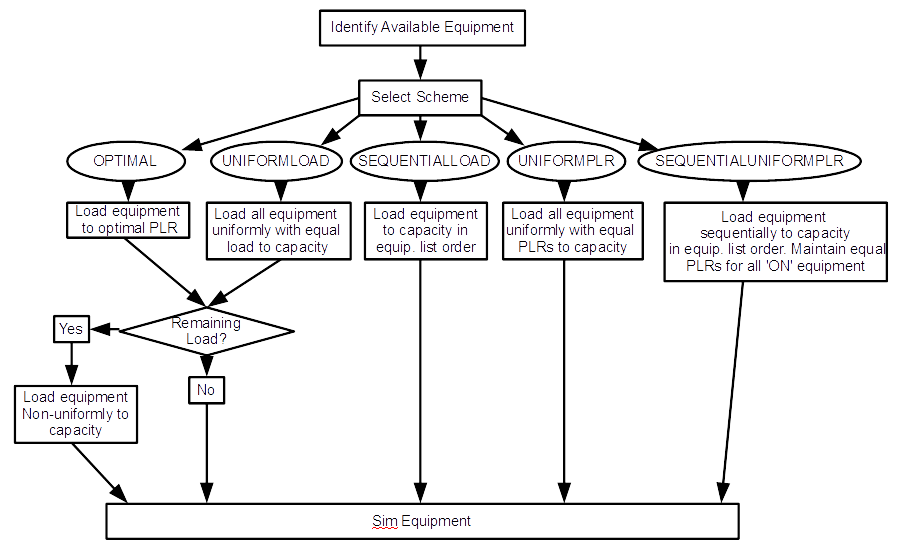
\includegraphics{media/image1974.png}

Figure 124. Load Distribution Scheme

The OPTIMAL scheme first loads each component to its optimal part load ratio (specified in input). Any remaining loop demand is distributed evenly to all the components. The UNIFORMLOAD scheme first divides the load evenly among all available components. If some components do not have the capacity to meet the uniformly distributed load, the remaining load is divided among the remaining components. The SEQUENTIALLOAD scheme loads each component one at a time to capacity until the loop demand is met. The components are loaded up in the order that they appear in the equipment list specified in input. The UNIFORMPLR scheme loads all equipment uniformly by maintaining uniform part load ratios across all equipment on the equipment list. If the load is below the load required by the plant to operate at the largest component minimum part load ratio, the last item is removed from each equipment list. This process is repeated until the plant can operate above the largest component minimum part load ratio. The SEQUENTIALUNIFORMPLR scheme loads all equipment in the order specified on the equipment list to capacity while operating all operational equipment at uniform part load ratios.

\emph{Note:} For all schemes, if the load for any individual component is less than the component load at the minimum PLR, the individual component model will false load or reduce duty cycle while operating at the minimum part load ratio until the load is met.

\subsection{Summary of Plant Loop Demand Calculation Schemes}\label{summary-of-plant-loop-demand-calculation-schemes}

There are two plant loop demand calculations schemes in EnergyPlus. There is a \textbf{SingleSetPoint} and a \textbf{DualSetPointDeadband}; the \textbf{SingleSetPoint} is the default if that field is left blank in the PlantLoop object. In the SingleSetPoint scheme the Plant Loop requires that a Setpoint Manager set a single setpoint value that sets Node\%TempSetPoint. Examples of this Setpoint Manager would be: the objects SetpointManager:Scheduled, SetpointManager:OutdoorAirReset, etc. For the DualSetPointDeadband scheme the Plant Loop requires that a Setpoint Manager that sets the high and low setpoint values for Node\%TempSetPointHi and Node\%TempSetPointLo. Examples of this setpoint manager would be: SetpointManager:Scheduled:DualSetpoint. Look in the Input Output Reference for the correct usage of these SetpointManagers.

The Plant Loop Demand Calculation Scheme determines the amount of heating or cooling necessary to bring the temperature of the Plant Loop to its setpoint(s). When this value is determined then the Load Distribution scheme explained in the previous section takes this value and distributes the load to the appropriate equipment. The demand calculation scheme determines how the load is calculated. In the next section is a summary of the 2 algorithms and how they are used.

\subsubsection{Loop Demand Calculation Scheme SingleSetPoint}\label{loop-demand-calculation-scheme-singlesetpoint}

The SingleSetPoint scheme for the PlantLoop takes the value that is placed on the Node\%TempSetPoint and calculates the heating or cooling load necessary to obtain that setpoint.

~~~~~~~ DeltaTemp~~~ = LoopSetPoint - LoopTempIn

~~~~~~~ LoopDemand = mdot * Cp * DeltaTemp

The sign of the Loop Demand determines if the loop has a cooling or heating load. Then the Load Distribution scheme distributes this calculated load to the appropriate equipment.

\subsubsection{Loop Demand Calculation Scheme DualSetPointDeadband}\label{loop-demand-calculation-scheme-dualsetpointdeadband}

The DualSetPointDeadband scheme for the PlantLoop takes the value that is placed on the Node\%TempSetPointHi and Node\%TempSetPointLo calculates the heating or cooling load necessary to obtain that setpoint; if in the DeadBand then no load is calculated. The pseudo code below shows the basis of the algorithm.

\begin{lstlisting}
        !Calculate the demand on the loop
        IF (mdot > 0.0) THEN
          LoadtoHeatingSetPoint = mdot*Cp*(LoopSetPointLo - LoopTempIn)
          LoadtoCoolingSetPoint = mdot*Cp*(LoopSetPointHi - LoopTempIn)
          ! Possible combinations:
          ! 1  LoadToHeatingSetPoint > 0 & LoadToCoolingSetPoint > 0 -->  Heating required
          ! 2  LoadToHeatingSetPoint < 0 & LoadToCoolingSetPoint < 0 -->  Cooling Required
          ! 3  LoadToHeatingSetPoint < 0 & LoadToCoolingSetPoint > 0 -->  Dead Band Operation
          ! 4  LoadToHeatingSetPoint > 0 & LoadToCoolingSetPoint < 0 -->  Not Feasible
          IF (LoadToHeatingSetPoint .GT. 0.0 .AND. LoadToCoolingSetPoint .GT. 0.0) THEN
             LoopDemand = LoadToHeatingSetPoint
          ELSE IF (LoadToHeatingSetPoint .LT. 0.0 .AND. LoadToCoolingSetPoint .LT. 0.0) THEN
             LoopDemand = LoadToCoolingSetPoint
          ELSE IF (LoadToHeatingSetPoint .LT. 0.0 .AND. LoadToCoolingSetPoint .GT. 0.0) THEN
             LoopDemand = 0.0
          ELSE
             CALL ShowSevereError
          END IF
        ELSE
          LoopDemand = 0.0
        END IF
\end{lstlisting}

\begin{lstlisting}
        IF(ABS(LoopDemand) < LoopDemandTol) LoopDemand = 0.0
\end{lstlisting}

The sign of the Loop Demand determines if the loop has a cooling or heating load. Then the Load Distribution scheme distributes this calculated load to the appropriate equipment, if there is any.

\subsection{Plant and Condenser Equipment Operation Schemes}\label{plant-and-condenser-equipment-operation-schemes}

Plants and condenser loops must have some mechanism for controlling the operation of the loop and which equipment is available under different operating conditions. Once the Loop load is calculated by the return conditions from the demand side and using the loop setpoint, this load needs to be allocated to the supply equipment according to the users input. This is mainly done by the operation schemes.

Each operation scheme must have the type of operation scheme, its identifying name, and the schedule that defines its availability. The first scheme appearing in the list is given the highest priority; the second scheme has second highest priority, etc. In other words, if according to its schedule, the first operation scheme is available, then it is used by the simulation to define how the plant or condenser loop operates. If it is not available, the second operation scheme in the list is checked to see if it is available until the highest priority scheme that is also available is found. See the Input Output Reference for input field details.

\subsection{Plant Operation Schemes}\label{plant-operation-schemes}

See the Input Output Reference for input field details. The options for plant control schemes are:

\subsubsection{Uncontrolled Loop Operation}\label{uncontrolled-loop-operation}

The PlantEquipmentOperation:Uncontrolled scheme takes the full capacity of the supply equipment and cools or heats the loop accordingly. An example would be a cooling tower where the cooling tower would cool the condenser loop with all of its available capacity and not be limioted by a capacity range or setpoint. Uncontrolled loop operation simply specifies a group of equipment that runs `uncontrolled'. If the loop runs, this equipment will run also, unless turned off by the loop flow resolver to maintain continuity in the fluid loop.

\subsubsection{Cooling Load Range Based Operation or Heating Load Range Based Operation}\label{cooling-load-range-based-operation-or-heating-load-range-based-operation}

PlantEquipmentOperation:CoolingLoad (or PlantEquipmentOperation:HeatingLoad) defines the different ranges and which equipment list is valid for each range. In each trio, there is a lower limit for the load range, an upper limit for the load range, and a name that links to an equipment availability list (PlantEquipmentList). Load range operation is used when the loop load is calculated and then the equipment is selected in the proper range. This allows for the most efficient operation of the plant equipment or for the user to determine the most efficient plant configuration. When the equipment list has been deteremined then the load is allocated to the equipment in a manner selected by the user with ``Optimal or Sequential'' load distribution scheme. The load range based operation scheme has two statements associated with it: a main statement that defines the ranges that individual priority settings are valid and the lists of equipment that may be used for each range.

\subsection{Condenser Operation Schemes}\label{condenser-operation-schemes}

This is very similar to the plant operation schemes, but there are several more options avaible with the CondenserLoop. The condenser operation schemes apply to the equipment on the `supply side' of the condenser loop---pumps, cooling towers, ground coupled heat exchangers, etc. The keywords select the algorithm that will be used to determine which equipment is available for each time step. The `\emph{Range Based Operation'} schemes select a user specified set of equipment for each user specified range of a particular simulation variable. `\emph{Load} \emph{Range} \emph{Based'} ~schemes compare the demand on the condenser supply side with specified load ranges and associated equipment lists. `\emph{Outdoor\ldots{}Range Based'} schemes compare the current value of an environmental parameter with user specified ranges of that parameter. See the Input Output Reference for input field details.

\subsubsection{Uncontrolled Loop Operation}\label{uncontrolled-loop-operation-1}

The PlantEquipmentOperation:Uncontrolled scheme takes the full capacity of the supply equipment and cools or heats the loop accordingly. An example would be a cooling tower where the cooling tower would cool the condenser loop with all of its available capacity and not be limioted by a capacity range or setpoint. Uncontrolled loop operation simply specifies a group of equipment that runs `uncontrolled'. If the loop runs, this equipment will run also, unless turned off by the loop flow resolver to maintain continuity in the fluid loop.

\subsubsection{Cooling Load Range Based Operation or Heating Load Range Based Operation}\label{cooling-load-range-based-operation-or-heating-load-range-based-operation-1}

PlantEquipmentOperation:CoolingLoad (or PlantEquipmentOperation:HeatingLoad) statement defines the different ranges and which equipment list is valid for each range. In each trio, there is a lower limit for the load range, an upper limit for the load range, and a name that links to an equipment availability list (CondenserEquipmentList). Load range operation is used when the loop load is calculated and then the equipment is selected in the proper range. This allows for the most efficient operation of the plant equipment or for the user to determine the most efficient plant configuration. When the equipment list has been deteremined then the load is allocated to the equipment in a manner selected by the user with ``Optimal or Sequential'' load distribution scheme. The load range based operation scheme has two statements associated with it: a main statement that defines the ranges that individual priority settings are valid and the lists of equipment that may be used for each range.

\subsubsection{Outdoor Drybulb Range Based Operation, Outdoor Wetbulb Range Based Operation,~ Outdoor RHPercent Range Based Operation}\label{outdoor-drybulb-range-based-operation-outdoor-wetbulb-range-based-operation-outdoor-rhpercent-range-based-operation}

The various ``PlantEquipmentOperation:Outdoor*'' statements define the different ranges of the various environmental parameters and which equipment list is valid for each range. After the keyword and the identifying name, a series of data trios is expected. In each trio, there is a lower limit for the load range, an upper limit for the load range, and a name that links to an equipment availability list (the ``CondenserEquipmentList'').

\subsubsection{Outdoor Drybulb Temperature Difference Based Operation,. Outdoor Wetbulb Temperature Difference Based Operation}\label{outdoor-drybulb-temperature-difference-based-operation.-outdoor-wetbulb-temperature-difference-based-operation}

The various ``PlantEquipmentOperation:Outdoor*Difference'' statements control strategies help to control any condenser equipment based on the difference between a reference node temperature and any environmental temperature. For example a cooling tower can be controlled by a strategy, which looks at the difference between the tower inlet temperature and wet-bulb temperature. A difference range is specified for each equipment list.

\subsection{Primary-Secondary Loop Systems}\label{primary-secondary-loop-systems}

The method to simulate a primary-secondary system in EnergyPlus is termed Common Pipe.

\subsubsection{Common Pipe}\label{common-pipe}

Common pipe feature eliminates the need of specifying two different EnergyPlus loops each for Primary and Secondary half loops. Instead the user can set up the system as it is used in real life applications. A common pipe simulation requires that pumps be placed on both Demand (Secondary) and Supply (Primary) sides of the loop. A typical Common Pipe layout as used in EnergyPlus is shown in Figure~\ref{fig:transmitted-radiation-in-three-directions-for}. The major assumptions in the common pipe implementation are as follows:

\begin{itemize}
\item
  Pumps are placed on both demand and supply side of the loop.
\item
  Secondary pump flow rate can be less than, equal to or greater than the primary pump flow rate.
\item
  The flow at the inlet node of the half loop is equal to the flow at the outlet node of the half loop.
\item
  The pumps can have different schedules and any loop can be shut off when the other loop is still running.
\end{itemize}

\begin{figure}[hbtp] % fig 125
\centering
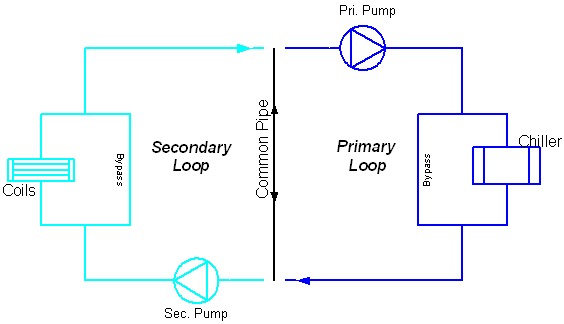
\includegraphics[width=0.9\textwidth, height=0.9\textheight, keepaspectratio=true]{media/image1975.png}
\caption{Common Pipe Layout Schematic \protect \label{fig:common-pipe-layout-schematic}}
\end{figure}

Common pipe simulation is done during the interface update call at both Supply-to-Demand and Demand-to-Supply. Appropriate checks are used to make sure that the effect of flow reversal in between iteration is taken care of. Moreover, the common pipe keeps track of the flow rates and temperatures at all the four nodes linked to it; namely, the inlet and outlet nodes of each sub loop. This record will help to decide if loops have converged or not. In situations where the primary component meets the setpoint and the coil controls does not change its flow request, the common pipe converges quickly. The simple description of the control algorithm for common Pipe implementation is as follows:

\begin{enumerate}
\def\labelenumi{\arabic{enumi}.}
\item
  At FirstHVACiteration, the common pipe flow is initialized to zero.
\item
  Common pipe is simulated at interfaces and thus we will have 2 different flows handle on either side of interface.
\item
  Loops and corresponding flow rates are assigned inlet or outlet (to common pipe) depending on the interface which calls it. So when common pipe is called from demand to supply interface, the inlet loop is demand side and outlet loop is supply side and vice versa.
\item
  Inlet flow is compared to outlet flow and the difference is set as the common pipe flow.
\item
  At each interface the common pipe flow is assigned a direction which can be into the interface (Inlet flow \textless{} Outlet flow) or away from interface (Inlet flow \textgreater{} Outlet flow).
\item
  Outlet temperature is calculated depending on the flow rate and flow direction. When flow is away from interface outlet flow temperature is same as inlet flow temperature. For a common pipe flow into the interface, the outlet flow temperature is calculated as mixed temperature of inlet flow and the common pipe flow.
\item
  At demand to supply interface, the supply side inlet node temperature and flow rate are updated every iteration. At supply to demand interface, only flow is updated. The temperature is updated only at the end of timestep.
\item
  Loops iterate till the flow and temperatures at all the 4 concerned nodes do not change.
\end{enumerate}

\subsubsection{Two-Way Common Pipe}\label{two-way-common-pipe}

A model referred to as Two-Way Common Pipe is available which provides a way to model Primary-Secondary systems as a single Plant Loop.~ In a typical EnergyPlus plant loop simulation, the only half loop inlet/outlet node that is controlled is the supply side outlet node. In some cases this requirement becomes a limitation in analyzing different options. A good example is ice thermal storage application, where during charging phase, the coil setpoint can be different from the ice storage equipment setpoint. With this model, the interface between the two half loops includes two additional flow paths that essentially split a single plant loop into both primary and secondary loop sides.~ Though the Two-Way common pipe is designed to be generic some assumptions apply in modeling the component. The assumptions are as follows

\begin{itemize}
\item
  The secondary flow may be less than, equal to, or greater than the primary flow.
\item
  The mass flow rate at the Primary Side Outlet Node is always equal to the mass flow rate at the Primary Side Inlet Node.
\item
  The mass flow rate at the Secondary Side Outlet Node is always equal to the mass flow rate at the Secondary Side Inlet Node.
\item
  Only one additional node, either primary-side inlet or secondary-side inlet, (along with the primary-side/supply-side outlet node) can be controlled. The system of equations that describe the loop interface will be under specified if both the Primary and Secondary Inlet nodes have to be controlled.
\end{itemize}

Figure~\ref{fig:schematic-of-a-two-way-common-pipe-used-in} shows a schematic of the Two-Way Common Pipe. There are two common pipe legs, shown as broken lines, allow for some recirculation at the half loop level.~ The model allows for common pipe flow in either or both directions. The model determines flow rates in the common pipes and temperatures at nodes based on the following:

\begin{itemize}
\item
  Which additional node is being controlled to meet a temperature setpoint? If the primary-side inlet node is controlled, then the flows are controlled to deliver the desired temperature at supply side inlet. If the secondary-side inlet node is controlled then the flows are controlled to deliver the desired temperature at the demand side inlet.
\item
  Is the specified setpoint achievable with current secondary and primary outlet conditions? If the setpoint is not achievable, then the flow in each common pipe leg is reduced to its minimum possible value.
\item
  At the controlled node, with known demand outlet temperature, supply outlet temperature, primary flow rate and secondary flow rate, and energy balance is used to calculate recirculation flows in the common pipes for that particular half loop, so that the desired temperature setpoint is achieved.
\item
  With a known flow in one common pipe leg, the flow on Primary to Secondary (or secondary to primary) is easily obtained by mass balance.
\item
  When the Two Way Common Pipe is controlling conditions at the secondary-side, or demand side, inlet node, then the loop capacitance model usually used for the conditions at the demand inlet is not used as it would interfere with control.
\end{itemize}

\begin{figure}[hbtp] % fig 126
\centering
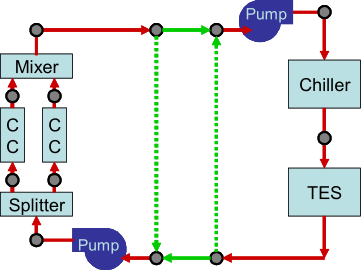
\includegraphics[width=0.9\textwidth, height=0.9\textheight, keepaspectratio=true]{media/image1976.svg.png}
\caption{Schematic of a Two-Way Common Pipe used in Primary-Secondary System. \protect \label{fig:schematic-of-a-two-way-common-pipe-used-in}}
\end{figure}

\subsection{Heat Recovery Loop Systems}\label{heat-recovery-loop-systems}

Heat Recovery is accomplished by specifying another set of supply and demand loops. Each of the heat recovery components, i.e.~engine driven and combustion turbine chillers, and internal combustion and combustion turbine generators is designed to use the existing component/loop/solution structure to facilitate the simulation with the existing demand side manager and the supply side manager. Heat recovery normally contains components that produce heat that can be recovered, and the ability to store or use that heat elsewhere in the system. The component that can store the excess heat and allow it to be used elsewhere in the system or for domestic hot water is the Water Heater:Simple and is defined in the Input/Output Reference.

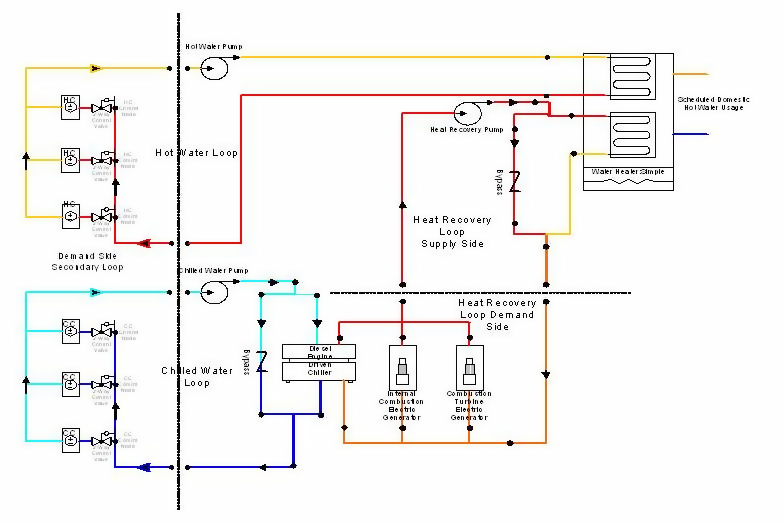
\includegraphics{media/image1977.png}.

Figure 127. Example of a Heat Recovery Loop Simulation

In the example above there is a chilled water Loop with chilled water supplied by a diesel engine driven chiller. There is a hot water Loop that is being supplied by the water heater: simple. There is also scheduled domestic hot water usage on the water heater which excess demand can be met by a number of user-specified heating sources. Then on the demand side of the heat recovery loop there is the engine driven chiller, internal combustion, and combustion turbine electric generators with specified mass flows to recover the heat. This hot water is pump on the supply side by the heat recovery pump and provides the heat to the water heater to meet the water heater setpoint. This is probably one of the more complex configurations and interactions that would take place in heat recovery, but using the Plant supply and demand side configurations this can be extended to meet most user configurations. The plant water heater can also be used to just meet scheduled domestic hot water use, provide a hot water source for PlantLoop equipment, or provide a hot water storage tank for heat recovery as a single function. Or any combination of the above can be configured. Example files of some of these configurations are provided with the installation.

\subsection{Plant Pressure Drop Simulation}\label{plant-pressure-drop-simulation}

As of version 4.0, there is an added feature which allows better calculation of pressure in plant and condenser loops. Without any method, the loops essentially ignore the node pressures. This is suitable for many applications, however may cause inaccuracies in the pump power. This is especially prominent in cases where the loop flow may change drastically over a wide range of configurations, as the pump power is based on a rated power value and rated pump head value. As the loop components turn on and off, the pressure drop will change, and so the pump power should be dynamically updated with these changes.

\subsubsection{Overall model features:}\label{overall-model-features}

Calculates loop pressure drop based on pressure drop information which is placed on branches. These are entered in terms of generic curves (linear, quadratic) or pressure drop information (minor loss/friction factor).

Loop pressure drop is used as the new pump head. No information is entered about the pump curve, so it is assumed that the pump will always be able to meet this operating point. Future enhancements will allow the pump to ride a curve based on the given pressure head.

Model does not resolve flow rates on parallel branches to match pressure drop, this is explained further below, but basically it takes the maximum pressure drop from parallel pressure components and applies that to all parallel components.

Model works for the following configurations:

\begin{enumerate}
\def\labelenumi{\arabic{enumi}.}
\item
  Pump Location
\item
  Loop Pump
\item
  Branch Pumps
\item
  Loop Types
\item
  PlantLoop
\item
  CondenserLoop
\end{enumerate}

The supply side inlet (before the pump) is always set to standard atmospheric pressure. This allows the node pressures around the loop to stay positive. The actual values of pressure are not all that important, it is the delta pressure that is of interest for our calculations, but this makes the pressure values appear realistic if one plots the pressure around the loop.

The pressure drop is at the branch level, not the component level. If multiple components are found on a single branch, the pressure drop is always applied to the last component on the branch. This is coordinated with the rule that a pump must always be the first component if it is found on a branch.

Calculations use the branch flow rate and the branch entering temperature to calculate properties for the whole branch.

\subsubsection{Detailed Restrictions:}\label{detailed-restrictions}

Pressure drop curves must not be placed on branches which only contain a pump. Pressure curves may be placed on the supply inlet branch with a pump as long as there are other components on that same branch, following the pump.

If using branch pumps, pressure drop curves found on the supply inlet branch will be ignored. Put pressure drop information after pumps.

Currently, pressure drop simulations are not allowed with common pipe (demand pump) simulations. A future version of the pressure drop system will allow this by allowing each pump to handle the pressure drop of the given loop side (demand or supply).

\subsubsection{Detailed Calculation Steps:}\label{detailed-calculation-steps}

Before the demand side is simulated, the pressure system is initialized. All node pressures are reset, and pressure drop values for branches are re-initialized.

After all components on a branch are simulated, the pressure drop for that branch is calculated. This pressure drop is registered in the pressure drop system to be used in subsequent loop level calculations.

Once the entire loop (demand then supply sides) is simulated, the loop level pressure drop calculations are performed using the following steps:

Beginning at demand side outlet (linked to supply inlet), and working backwards, the node pressure is updated and loop pressure is summed by ``adding pressure drops'' as they are found around the loop. By working backward, we are able to easily preserve the pump inlet pressure as a realistic value (standard atmospheric pressure).

When a parallel system is encountered, a special operation is performed. Since we are not resolving flows with this version of the pressure simulation, the parallel system is set to use the largest value of pressure drop found on the parallel branches. In this manner, the highest pressure drop component essentially governs the set of parallel branches, and the other components must match the pressure drop in order to achieve their desired flow rate. This is performed by placing ``imaginary'' valves in the splitter. This allows individual branches to report their own pressure information, while the splitter accounts for the required pressure drop to match the governing branch. This is shown graphically in the figure below.

\begin{figure}[hbtp] % fig 128
\centering
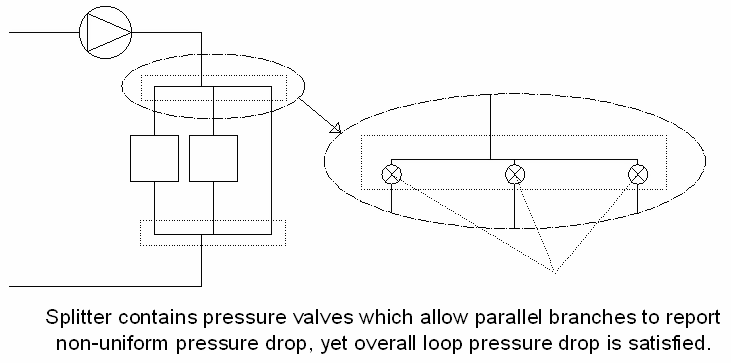
\includegraphics[width=0.9\textwidth, height=0.9\textheight, keepaspectratio=true]{media/image1978.png}
\caption{Explanation of valves inherently built into Splitter object \protect \label{fig:explanation-of-valves-inherently-built-into}}
\end{figure}

Because the splitter automatically handles the pressure drop required to match the pressures in the parallel system, the mixer will have uniform flow entering from all branches and exiting.

These calculations are performed around the loop and result in a value of pressure drop for the entire loop.

Pump power requires a value of pressure head before it can add heat to the loop, which is done before any components are calculated, and any pressure system calculations are performed. Because of this, the pump power is based on rated head during the first iteration. On subsequent iterations, the pump power is based on the dynamic pressure head calculated by pressure drop information.

If anything drastically changes between one iteration and the next, the loop will be re-simulated, and the latest value of pressure head will be used. By the time the loop is converged, the pressure head between the current and most previous iterations will agree to within simulation tolerance. Thus the pump is using a lagged value of pressure head, but once the loop is converged, the lagged and current values will agree.

\subsubsection{Pressure Drop Calculations:}\label{pressure-drop-calculations}

There are two types of pressure drop curves that can be entered, each with its own calculation engine:

Generic: A curve of any form (single independent variable) such as linear or quadratic may represent the pressure drop in Pascals as a function of current mass flow rate in kg/s. This is common for regressing component pressure drop such as heat pumps into a quadratic best fit form. The branch pressure drop is then calculated by evaluating this curve with the given branch flow rate.

Pressure Information: This calculation involves two types of pressure drop: frictional effects and minor losses. The governing equation is:

\begin{equation}
\Delta P = \left( {f\frac{L}{D} + K} \right)\frac{{\rho {V^2}}}{2}
\end{equation}

The user enters value for the minor loss coefficient K to represent all the minor losses on that branch. If the user is entering friction information, the minor loss coefficient may be zero or blank.

The user enters roughness, e, or a fixed value of friction factor to account for frictional losses on the branch, as well as an equivalent length L. If the user enters roughness then the friction factor is calculated from a Moody chart approximation (Haaland, 1983):

\begin{equation}
f = {\left\{ { - 1.8\log \left[ {{{\left( {\frac{{e/D}}{{3.7}}} \right)}^{1.11}} + \frac{{6.9}}{{{\mathop{\rm Re}\nolimits} }}} \right]} \right\}^{ - 2}}
\end{equation}

If the user enters minor loss information, then the friction factor information can be left out.

The diameter is an equivalent value and is used to calculate relative roughness for friction calculations as well as velocity for any pressure drop calculation.

\subsubsection{Riding Pump Curves to Determine Loop Operating Point}\label{riding-pump-curves-to-determine-loop-operating-point}

In addition to being able to provide a means of calculating loop pressure drop, EnergyPlus can also perform a ``loop-level'' pump-system flow resolution.~ The pressure drop components that were described in the previous sections are combined with the input of a dimensionless pump pressure-flow curve and at each iteration, these are utilized in determining a proper operating point for the loop.

Some restrictions do apply to this simulation.~ As with the basic pressure drop simulation, common pipes are not valid in the current release.~ For this pump curve phase, the simulation is also restricted to ``loop pumps'' such that pumps should not be used on the parallel branches between a mixer and splitter.

The idea of riding a pump curve, as it is currently implemented, is based on a constant speed pump.~ A variable speed pump in EnergyPlus can already effectively vary its flow/pressure characteristics to meet the demand.~ Thus, this phase is only implemented for the Pump:ConstantSpeed model.

The model works by approximating the loop with a quadratic pressure drop form, then iterating to find an operating point.~ The entire plant loop then iterates to find the operating point that attempts to match the requested flows.~ Note that when doing a pressure based pump simulation, the loop will likely not hit setpoint every timestep, while doing the simpler approach (non-pressure) may result in a tighter-controlled simulation.~ In deciding this, you must consider the realism of the pressure approach vs.~the non-pressure approach which may be more tightly controlled and will have less input requirements.

In the first iteration of the plant, there is not yet enough information to determine a pressure-flow simulation, so flow through the loop is set to the rated flow rate of the pump (irrespective of pump performance curve). For this rated flow rate pressure drop in each branch will be calculated by plant pressure system. So after this first pass through the loop, the pressure system now has a valid system flow-pressure point.~ From this point (pressure drop in the branch and rated mass flow rate) a pressure constant for each branch is calculated assuming quadratic relationship between pressure drop and mass flow rate.

\begin{equation}
{K_{Branch(i)}} = \Delta {P_{Branch(i)}}/{m_{Rated}}^2
\end{equation}

If there are parallel branches then equivalent K is calculated from following formula.

\begin{equation}
\frac{1}{{\sqrt {{K_{ParallelEquivalent}}} }} = \sum\limits_{j = 1}^m {\frac{1}{{\sqrt {{K_{Branch(j)}}} }}}
\end{equation}

From all these `K' values of the branches a corresponding K value for complete loop is calculated. This representative K value for the loop will lock down a system curve for a single iteration.~ This K value will change throughout the higher-level plant iterations and simulation time steps.

The Non-dimensional pump curve is entered in following way,

\begin{equation}
\psi  = {C_4} \times {\varphi ^4} + {C_3} \times {\varphi ^3} + {C_2} \times {\varphi ^2} + {C_1} \times \varphi  + {C_0}.
\end{equation}

C\(_{1-4}\) are curve coefficients with last mandatory non-zero constant term C\(_{0}\) (as pump curve will not pass through origin).

The nondimensional variables in the previous equation are defined in terms of the following expressions:

Ψ -- Non-dimensional pressure rise:~ \(\psi = \frac{{\Delta P}}{{\rho {N^2}{D^2}}}\)

φ - Non-dimensional flow:~ \(\varphi = \frac{{\dot m}}{{\rho N{D^3}}}\)

The user preprocesses mass flow and pressure values into these nondimensional forms in order to generate the curve fit.~ The program then resolves the nondimensional forms into actual values based on the pump speed, diameter, and fluid density.~ This gives the proper pressure-flow relationship for the simulation.

\subsubsection{Pump-System Operating Point Flow Resolver:}\label{pump-system-operating-point-flow-resolver}

The pressure drop components and the pump curve are described in the prior sections.~ The routine which actually uses these curves to resolve to an operating point is described here.~ This routine is called by the pump model as it is determining what flow it should be using.~ The flow resolver reads the non-dimensional pump curve, loop pressure constant (K value) and rated mass flow rate (or mass flow rate from last iteration). The resolver finds the intersection of the two curves by successive substitution with 0.9 as a damping factor. If the flow rate is outside (or if in any iteration move out of) the range for which pump curve-fit is suggested, the resolver will bring the value within range, thus it is important to specify the curve-fit range (in terms of non-dimensional flow rate) for pump curve by the user.~ It was observed that simple successive substitution (sometimes) diverges depending on shape of curves and/or location of operating point. Damping factor provides stability to successive substitution and it was observed that it converges for less number of iteration, speeding up the function. The damping factor was set as 0.9 as it showed full stability during testing, although a more optimum value may be available for a particular set of curves.~ A future version may have an improved selection algorithm for the damping factor itself.

\subsubsection{References}\label{references-037}

Haaland, SE. 1983. ``Simple and Explicit Formulas for the Friction Factor in Turbulent Flow''. Transactions ASIVIE, Journal of Fluids Engineering 103: pp.~89-90.
